%%%%%%%%%%%%%%%%%%%%%%%%%%%%%%%%%%%%%%%%%%%%%%%%%%%%%%%%%%%%%%%%%%%%%%%%

%%% LaTeX Template for AAMAS-2027 (based on sigconf.tex)
%%% Prepared by the AAMAS-2027 Publication Chairs based on the version from AAMAS-2026. 

%%%%%%%%%%%%%%%%%%%%%%%%%%%%%%%%%%%%%%%%%%%%%%%%%%%%%%%%%%%%%%%%%%%%%%%%

%%% Start your document with the \documentclass command.
%%%
%%% VERSION FRANCAISE de l'article court, AAMAS 2027. Gabarit officiel AAMAS-2027 fourni par
%%%   l'auteur le 22 septembre 2026, avec quatre changements et rien d'autre :
%%%   1. titre et mots-cles de l'article court, en francais ;
%%%   2. babel french et emergencystretch (voir plus bas) ;
%%%   3. le \section{Citations and References} d'exemple est retire : il s'imprimerait en
%%%      section vide apres le 7 ;
%%%   4. le texte d'exemple des acks est commente (consigne R14).
%%%
%%% L'ANGLAIS FAIT FOI (consigne R17, decision de l'auteur du 22 septembre 2026). Cette
%%%   version est un rendu : les chapitres viennent de ../sections/*.fr.md, qui se
%%%   realignent eux-memes sur les *.en.md. Une correction de fond se fait en anglais.


%%% == IMPORTANT ==
%%% Use the first variant below to anonymize your submission (no author information shown).
%%% Use the second variant below for the final paper (including author information).
%%% For further information on anonymity and double-blind reviewing, 
%%% please consult the call for paper information
%%% https://warwick.ac.uk/fac/sci/dcs/aamas2027/calls/

%%%% For anonymized submission, use this
\documentclass[sigconf,anonymous]{aamas} 
\renewcommand{\texttt}[1]{{\ttfamily\hyphenchar\font=`\-\relax\hyphenpenalty=10000\relax #1}}
%%%% For camera-ready, use this
%\documentclass[sigconf]{aamas} 


%%% Load required packages here (note that many are included already).

\usepackage{balance}  % for balancing columns on the final page
\usepackage{tikz}
\usetikzlibrary{arrows.meta, positioning, shapes.geometric}
\usepackage{array}    % >{...} column prefixes, needed by the L column below
\usepackage{tabularx} % width-constrained tables
\usepackage{afterpage}% deferred \clearpage, float flushing at chapter boundaries
\newcolumntype{L}{>{\raggedright\arraybackslash}X}
\newcommand{\todo}[1]{\textbf{[#1]}}

%%% LANGUE. babel french charge sans conflit sous aamas.cls : il pose seul l'espace fine
%%%   insécable devant ; : ! ?, gère les guillemets et traduit References en Références.
%%%   Ne pas doubler l'espace à la main dans les chapitres.
\usepackage[french]{babel}

%%% JUSTIFICATION. Le français fait des mots plus longs : cinq paragraphes débordaient dans
%%%   la gouttière, jusqu'à 18,5 pt. \emergencystretch laisse TeX détendre ces lignes-là.
%%%   Ne touche ni les marges, ni le corps, ni l'interligne.
\emergencystretch=1.5em

\setcounter{topnumber}{3}
\setcounter{bottomnumber}{2}
\setcounter{totalnumber}{4}
\setcounter{dbltopnumber}{2}
\renewcommand{\topfraction}{0.85}
\renewcommand{\dbltopfraction}{0.85}
\renewcommand{\bottomfraction}{0.5}
\renewcommand{\textfraction}{0.1}
\renewcommand{\floatpagefraction}{0.75}
\renewcommand{\dblfloatpagefraction}{0.75}

%%%%%%%%%%%%%%%%%%%%%%%%%%%%%%%%%%%%%%%%%%%%%%%%%%%%%%%%%%%%%%%%%%%%%%%%

%%% AAMAS-2027 copyright block (do not change!)

\makeatletter
\gdef\@copyrightpermission{
  \begin{minipage}{0.2\columnwidth}
   \href{https://creativecommons.org/licenses/by/4.0/}{
\includegraphics[width=0.90\textwidth]{by}}
  \end{minipage}\hfill
  \begin{minipage}{0.8\columnwidth}
   \href{https://creativecommons.org/licenses/by/4.0/}{This work is licensed under a Creative Commons Attribution International 4.0 License.}
  \end{minipage}
  \vspace{5pt}
}
\makeatother

\setcopyright{ifaamas}
\acmConference[AAMAS 2027]{Proc.\@ of the 26th International Conference
on Autonomous Agents and Multiagent Systems (AAMAS 2027)}{3--7 May 2027}{Hanoi, Vietnam}{M.~Baldoni, F.~Fang, W.~Yeoh, N.~Yorke-Smith (eds.)}
\copyrightyear{2027}
\acmYear{2027}
\acmDOI{}
%\acmPrice{}
\acmISBN{}

%%%%%%%%%%%%%%%%%%%%%%%%%%%%%%%%%%%%%%%%%%%%%%%%%%%%%%%%%%%%%%%%%%%%%%%%

%%% == IMPORTANT ==
%%% Use this command to specify your OpenReview submission number.
%%% In anonymous mode, it will be printed on the first page.

\acmSubmissionID{<<OpenReview submission id>>}

%%% Use this command to specify the track you want to submit your paper to.

\submissionType{Research Paper Track}
%\submissionType{AAAI Track}
%\submissionType{Demonstration Track}
%\submissionType{Blue Sky Ideas Track}
%\submissionType{JAAMAS Track}
%\submissionType{Doctoral Consortium}

%%% Use this command to specify the title of your paper.

\title[Là où le chain-of-thought mérite sa place]{Là où le chain-of-thought mérite sa
place : des agents génératifs de mobilité face à une enquête ménages déplacements réelle}

%%% Provide names, affiliations, and email addresses for all authors.

\author{Yves Bru}
\affiliation{
  \institution{UMR IRIT, Université Toulouse Capitole}
  \city{Toulouse}
  \country{France}}
\email{yves.bru@gmail.com}

\author{Benoit Gaudou}
\affiliation{
  \institution{UMR IRIT, Université Toulouse Capitole}
  \city{Toulouse}
  \country{France}}
\email{benoit.gaudou@ut-capitole.fr}

\author{Kamaldeep Singh Oberoi}
\affiliation{
  \institution{CESI, CESI LINEACT}
  \city{Toulouse}
  \country{France}}
\email{ksoberoi@cesi.fr}

%%% Use this environment to specify a short abstract for your paper.

% =====================================================================
% chapters/00_Abstract.tex — rendu LaTeX de ../traductions/00_abstract.en_brut.txt (23 septembre 2026)
% Chapitre 0 de la VERSION FRANÇAISE de l'article court : le résumé. \input depuis main.tex,
%   dans le préambule, avant \begin{document}, comme le fait le gabarit AAMAS.
% Rendu mot pour mot de la traduction fournie par l'auteur.
% TYPOGRAPHIE : babel french pose seul l'espace fine devant ; : ? !
%   Ce qui est explicite ici : 1\,000 et 3\,299 (séparateur de milliers en espace fine
%   insécable), la virgule décimale étant un simple caractère.
% NOTE DE BAS DE PAGE : préservée sur l'enquête CEREMA 2023.
% =====================================================================

\begin{abstract}
Les simulations multi-agents de mobilité urbaine choisissent les modes de transport à l'aide de modèles tabulaires ajustés à partir d'enquêtes sur les déplacements déclarés, ou à l'aide de règles élaborées par des experts du domaine. Ces deux approches fixent l'espace des comportements représentables avant le lancement de la simulation ; ainsi, un facteur non pris en compte par une variable ou une règle n'influence aucune décision. Les agents génératifs construits sur des modèles de langage promettent de lever cette contrainte, en intégrant des heuristiques de décision que les enquêtes n'enregistrent jamais. À notre connaissance, la validité de cette promesse face à une population réelle n'a pas encore été vérifiée.

Nous l'évaluons sur la région toulousaine, en nous appuyant sur l'enquête certifiée CEREMA 2023 sur les déplacements des ménages\footnote{Enquête Ménages Déplacements (EMD), Toulouse / Grande agglomération toulousaine --- 2023, CEREMA, Syndicat mixte des transports en commun de l'agglomération toulousaine (producteurs), PROGEDO-ADISP (diffuseur). Rapport final : \url{https://www.aua-toulouse.org/wp-content/uploads/2024/05/Rapport-final-68-pages-Enquete-mobilite-2023-Bassin-de-vie-toulousain.pdf}}. Une cohorte fermée de 1\,000 profils synthétiques, contrôlés par rapport à treize marges de cette enquête, effectue les 3\,299 déplacements du jour que nous analysons. Quinze décideurs effectuent ces déplacements selon un protocole unique. Ce protocole leur fournit les mêmes 21 variables d'entrée. Il calcule la probabilité que chaque décideur attribue à chaque option proposée.

En ajustant l'invite pour mettre en évidence des critères généraux (tels que le confort, les contraintes ou les opportunités liées au choix d'une option), l'agent génératif se rapproche des caractéristiques des modèles tabulaires. Aucun de nos agents ne les atteint. Un classificateur qui lit le même contexte avec un type de sortie fixe et n'écrit aucun texte, les égale pour un cinquantième du coût. L'agrégat masque ce qu'une lecture au niveau de la décision révèle. Deux décideurs que l'agrégat ne peut distinguer sont en désaccord sur un trajet sur trois. Le classificateur se trompe sur plus de trajets individuels qu'une règle qui ne lit rien.

La délibération verbalisée trouve sa place en dehors du quotidien. Chez un agent, une panne de moteur est entrée dans la mémoire, a dissuadé l'utilisation de la voiture pendant quinze jours, puis s'est estompée. Aucun décideur ne disposant que des 21 variables ne peut répondre à un tel événement. Nos mesures encouragent l'utilisation du modèle de langage lorsque les événements surviennent et laissent le quotidien à un décideur qui ne délibère pas.
\end{abstract}


%%% Use this command to specify a few keywords describing your work.
%%% Keywords should be separated by commas.

\keywords{Agents génératifs ; Modèles de langue ; Simulation multi-agents ;
Mobilité urbaine ; Choix modal ; Calage sur enquête déplacements}

%%%%%%%%%%%%%%%%%%%%%%%%%%%%%%%%%%%%%%%%%%%%%%%%%%%%%%%%%%%%%%%%%%%%%%%%

%%% Include any author-defined commands here.
         
\newcommand{\BibTeX}{\rm B\kern-.05em{\sc i\kern-.025em b}\kern-.08em\TeX}

%%%%%%%%%%%%%%%%%%%%%%%%%%%%%%%%%%%%%%%%%%%%%%%%%%%%%%%%%%%%%%%%%%%%%%%%

\begin{document}

%%% The following commands remove the headers in your paper. For final 
%%% papers, these will be inserted during the pagination process.

%\pagestyle{fancy}
%\fancyhead{}

%%% The next command prints the information defined in the preamble.

\maketitle 

%%%%%%%%%%%%%%%%%%%%%%%%%%%%% CHAPTERS %%%%%%%%%%%%%%%%%%%%%%%%%%%%%%%%%%%%%%%%%%%

% =====================================================================
% chapters/01_Introduction.tex — rendu LaTeX de ../traductions/01_introduction.en_brut.txt (23 septembre 2026)
% Section 1 de la VERSION FRANÇAISE de l'article court. \input depuis main.tex, première du corps.
% Ce fichier DÉFINIT \label{sec:intro}. La section 1.4 renvoie à toutes les autres sections :
%   elle porte six \ref.
% Citations : lammer2026gta (GTA), vu2025modeling (architecture), tisseo2023emc2 (enquête).
% Rendu mot pour mot de la traduction fournie par l'auteur.
% =====================================================================

\section{Introduction}
\label{sec:intro}

\subsection{Les promesses des agents génératifs}
\label{sec:promise}

Les simulations multi-agents existantes de mobilité urbaine multimodale reposent sur des modèles tabulaires estimés à partir d'enquêtes de mobilité des ménages, ou sur des règles explicites définies par des experts du domaine. Une enquête de mobilité des ménages demande aux habitants d'un territoire de décrire chaque déplacement effectué au cours d'une journée. Dans les deux cas, l'espace des comportements représentables est fixé \emph{a priori} ; un facteur n'étant ni une variable ni une règle ne peut influencer aucune décision.

Cet espace comportemental fixe limite précisément le domaine où la simulation est censée intervenir. Une ville teste une politique de transport sur une population simulée avant d'entreprendre toute construction. Le résultat obtenu est limité par le comportement que son modèle peut représenter. Le choix du mode de transport étant multidimensionnel, intégrer cette complexité à l'échelle de la ville est difficile.

Les agents génératifs construits sur des modèles de langage promettent de surmonter cette difficulté. Alimentés par des corpus massifs, ils intègrent des heuristiques de décision que les enquêtes n'enregistrent pas et s'adaptent sans règles explicites. Une grève, une vague de chaleur ou un article de presse sur la sécurité dans le métro pourraient alors aboutir à une décision qu'aucune enquête ne permet de prendre. Ces systèmes promettent également de fonctionner sans les données d'étalonnage locales requises par les modèles à base d'agents. Des ensembles de données détaillés sur les trajectoires multimodales existent uniquement pour quelques grandes métropoles.

\subsection{Évaluation des promesses face à une population réelle}
\label{sec:gap}

Les évaluations publiées de ces agents font rarement l'objet d'une comparaison avec une population humaine. La plupart évaluent un agent génératif par rapport à un agent basé sur des règles, ou par rapport à des modèles agrégés produits par les auteurs eux-mêmes. Un système se distingue.

GTA \citep{lammer2026gta} confronte une répartition modale simulée à une enquête nationale sur les déplacements. La répartition modale correspond à la part des déplacements effectués par chaque mode. GTA crée ses personas à partir de cette enquête. Un modèle de langage rédige le plan de journée de chacun. Sa seule référence modélisée est la répartition observée dans d'autres régions. Copier les parts de Hambourg génère une erreur quadratique moyenne de 1,99 sur Berlin, contre 4,07 pour sa propre simulation.

Cet article apporte quatre éléments manquants à ces comparaisons. Une ligne de base sous les agents indique la décision qu'un décideur prendrait sans connaissance comportementale du territoire. Les modèles ajustés sur l'enquête propre à ce territoire indiquent ce que confirment ses données. Les mêmes entrées des deux côtés créent un écart attribuable au décideur plutôt qu'aux informations qui lui ont été communiquées. Une lecture sous l'agrégat indique si deux décideurs produisant les mêmes parts prennent des décisions similaires.

\subsection{Ce que fait cet article}
\label{sec:contributions}

Cet article mesure la pertinence de la délibération verbalisée dans un agent de mobilité. La délibération verbalisée consiste pour le modèle à formaliser son raisonnement par écrit avant de répondre. Dans une population d'agents de mobilité, elle n'améliore pas la fidélité au régime ordinaire décrit par l'enquête. Elle introduit des événements qu'aucune variable n'encode. Nous retraçons le parcours d'un tel événement jusqu'à la décision.

Nous effectuons des mesures sur un territoire, la région toulousaine, en nous basant sur son enquête certifiée sur les déplacements des ménages de 2023 \citep{tisseo2023emc2}. Un groupe contrôlé de 1\,000 profils synthétiques effectue les 3\,299 déplacements du jour que nous analysons. Quinze décideurs interviennent sur ces déplacements. Nous appelons «~décideur~» tout agent qui transforme la description d'un déplacement en une probabilité parmi les options proposées. Les agents évoluent dans une simulation multi-agents GAMA de la région toulousaine, avec ses réseaux et horaires réels. Cette simulation suit l'architecture GAMA--OpenTripPlanner--LLM de \citet{vu2025modeling}.

Cet article repose sur trois contributions. La première est un banc d'essai comparatif avec des entrées égales entre agents génératifs et modèles tabulaires, sur une cohorte synthétique contrôlée par rapport à cette enquête. La seconde concerne la position de quinze décideurs sur ce banc d'essai, et deux dissociations que les parts agrégées ne révèlent pas. Le troisième point concerne le parcours d'un événement non tabulé jusqu'à la décision, au sein d'un agent génératif doté de mémoire.

\subsection{Organisation}
\label{sec:organisation}

Cet article suit l'ordre de la mesure. La section~\ref{sec:related} le situe dans trois contextes bibliographiques. La section~\ref{sec:agent} décrit ce que l'agent évalué reçoit et renvoie. La section~\ref{sec:bench} présente le banc de comparaison et son protocole. La section~\ref{sec:results} décrit une journée type. La section~\ref{sec:nontabulated} analyse l'événement non tabulé. La section~\ref{sec:implications} en tire les implications, les limites et la conclusion.

% =====================================================================
% chapters/02_Related_work.tex — rendu LaTeX de ../traductions/02_related_work.en_brut.txt (23 septembre 2026)
% Section 2 de la VERSION FRANÇAISE de l'article court. \input depuis main.tex, après 01_Introduction.tex.
% Ce fichier DÉFINIT \label{sec:related}, visé par la carte de lecture de la section 1.4.
% Citations : mcfadden1974conditional, benakiva1985discrete, train2009discrete, verplanken1997habit,
%   garling2003habitual, adam2025survey, park2023generative, liu2024toward, bougie2025citysim,
%   horni2016matsim, lammer2026gta, alves2026evaluating, argyle2023outofone, meister2024benchmarking,
%   baronchelli2025emergent, bintareaf2026silica, wei2022chain, sprague2024cot.
% Rendu mot pour mot de la traduction fournie par l'auteur.
% =====================================================================

\section{Travaux connexes}
\label{sec:related}

Trois courants de recherche se rejoignent dans cet article, et aucun n'évalue si la délibération verbalisée aide les agents à reproduire les parts modales d'un territoire réel.

\subsection{Choix discret et filtres de perception}
\label{sec:discrete-choice}

Depuis cinquante ans, la recherche en transport prédit le choix modal à l'aide de modèles de choix discret, statistiquement robustes et comportementalement rigides. Un tel modèle attribue à chaque mode une probabilité calculée à partir du temps de trajet, du coût et des caractéristiques du voyageur \citep{mcfadden1974conditional,benakiva1985discrete}. Les analystes l'ajustent aux enquêtes de mobilité, dans lesquelles les résidents décrivent chaque trajet d'une journée, de sorte qu'il hérite de leurs parts modales \citep{train2009discrete}. Sa règle de décision, cependant, est une maximisation sur des distributions fixes de préférences.

La recherche comportementale documente des départs qu'aucune enquête n'enregistre. L'habitude rend un choix modal répété automatique. Le voyageur acquiert alors moins d'informations sur les alternatives \citep{verplanken1997habit,garling2003habitual}. \citet{adam2025survey} ont interrogé 650 personnes et ont constaté que les automobilistes réguliers sous-estimaient le prix d'une voiture. Comme un modèle basé sur des enquêtes ne peut intégrer de tels filtres de perception, les agents génératifs sont proposés pour combler cette lacune.

\subsection{Agents génératifs dans la simulation de mobilité}
\label{sec:generative-mobility}

Les modèles de langage ont fait leur apparition dans la simulation de mobilité en tant que composante délibérative absente des simulateurs précédents. \citet{park2023generative} placent le modèle au sein de l'agent, avec une mémoire épisodique et une capacité de réflexion. \citet{liu2024toward} transposent cette approche à la demande de transport, sous forme d'hybride avec des composantes établies. CitySim \citep{bougie2025citysim} déploie ces agents à l'échelle d'une ville et les valide en fonction de l'utilisation du temps. Aucune expérience ne confronte une répartition modale simulée à une répartition modale observée. Dans les simulateurs antérieurs tels que MATSim \citep{horni2016matsim}, l'équilibre résulte de la notation des plans plutôt que de la délibération d'un agent.

GTA \citep{lammer2026gta} est le système publié le plus proche en termes d'évaluation, et trois de ses choix limitent ce qu'il peut afficher. Chaque agent renvoie un mode par trajet plutôt qu'une distribution, donc aucune métrique distributionnelle ne s'applique. Ses jours sont également indépendants. Ses auteurs mentionnent la mémoire multi-jours comme travaux futurs. Nous ajoutons une ligne de base sous les agents et quatre modèles ajustés sur l'enquête au-dessus. Notre métrique évalue une distribution complète, et non un mode par trajet. Nos agents conservent les événements d'un jour à l'autre.

\citet{alves2026evaluating} sont les plus proches du point de vue de la plateforme, bien que leur évaluation ne repose sur aucune vérité humaine. Ils couplent la plateforme GAMA à un module de modélisation du langage doté d'une mémoire persistante, qui détermine, en cas de perturbation, si un agent doit replanifier. Ils évaluent l'adaptabilité par rapport à une base de référence fondée sur des règles, et non par rapport au comportement observé.

\subsection{Alignement distributionnel des populations de modèles de langage}
\label{sec:alignment}

Une autre littérature s'interroge sur la possibilité pour les populations de modèles de langage de se substituer à des échantillons humains. \citet{argyle2023outofone} ont conditionné un modèle sur des attributs sociodémographiques et ont retrouvé les schémas de réponse de la sous-population correspondante. \citet{meister2024benchmarking} ont constaté qu'un modèle verbalisant une distribution s'aligne mieux que le même modèle échantillonné de manière répétée. Notre protocole évalue une distribution verbalisée pour cette raison.

Cette même littérature met en garde contre l'interprétation de ces populations comme étant des populations humaines. \citet{baronchelli2025emergent} constatent des biais collectifs dans les populations de modèles décentralisés, biais qu'aucun agent individuel ne présente. Ils refusent leur statut de substitut humain. L'instrument SILICA \citep{bintareaf2026silica} certifie ces populations à l'aide d'une bibliothèque de perturbations, incluant l'ordre des options. Nous adoptons sa grille de lecture et son contrôle de l'ordre des options.

L'utilité de rédiger le raisonnement avant de répondre fait débat, aucun résultat ne permettant de trancher la question pour une distribution de population donnée. Les gains observés pour le raisonnement écrit proviennent de tâches qui admettent une réponse vérifiable \citep{wei2022chain,sprague2024cot}. Nous effectuons donc nos mesures sur une population d'agents de mobilité, dont la boucle est décrite dans la section suivante.

% =====================================================================
% chapters/03_Agent.tex — rendu LaTeX de ../traductions/03_agent.en_brut.txt (23 septembre 2026)
% Section 3 de la VERSION FRANÇAISE de l'article court. \input depuis main.tex, après 02_Related_work.tex.
% Ce fichier DÉFINIT \label{sec:agent} et \label{sec:memory}.
% Figure : une, figure* sur les deux colonnes (architecture_GAMA_Agents.jpg), légende AU-DESSOUS.
% Rendu mot pour mot de la traduction fournie par l'auteur.
% =====================================================================

\section{L'agent évalué}
\label{sec:agent}

Chaque agent transforme la description d'un trajet en une préférence parmi les options proposées. Cette section décrit ce que l'agent reçoit, ce qu'il renvoie, ainsi que les deux mécanismes testés dans cet article : la masse de probabilité et la mémoire.

\subsection{La boucle}
\label{sec:loop}

La simulation repose sur trois composants. Une simulation multi-agents GAMA modélise le monde : la géographie réelle des 453 communes, les réseaux, l'horloge et l'exécution physique de chaque trajet. OpenTripPlanner génère les itinéraires de transport public à partir des horaires réels. Un calcul du plus court chemin sur le graphe OpenStreetMap détermine les trajets directs à pied, à vélo et en voiture. Un contrôleur gère le cycle de vie de l'agent et construit les options disponibles à l'heure de départ. Un module de décision effectue le choix. Le modèle de langage est appelé à trois moments de la boucle : la décision, la consolidation de la mémoire en fin de journée et une auto-réflexion sur plusieurs jours. Cet article teste la décision.

\begin{figure*}[tp]
  \centering
  
\includegraphics[width=\textwidth]{images/architecture_GAMA_Agents.jpg}
  \caption{Les trois composantes de la boucle. Cet article teste le module de décision.}
  \Description{Schéma fonctionnel du dispositif, sur trois bandes horizontales. Bande supérieure, l'agent génératif : groupe d'icônes d'agents relié à gauche à une boîte passerelle LLM (rotation des fournisseurs, cache), à droite à deux boîtes (planification des activités quotidiennes et planification des déplacements), et en dessous à deux mémoires (mémoire à court terme et mémoire à long terme), reliées par une flèche réflexion ; une double flèche entre les agents et les mémoires indique la lecture et l'écriture en mémoire. Deux boîtes en tiretés alimentent l'agent par le haut : données de population (identité personnelle, activités journalières) et environnement (météo, trafic). Bande médiane, une barre horizontale échange de données, avec les services Python au-dessus et GAMA en Java en dessous ; les perceptions montent par HTTP vers la mémoire à court terme, les actions descendent par WebSocket. Bande inférieure, la plateforme GAMA : carte du réseau toulousain et icônes bus, train, tramway, téléphérique, vélo, marche et voiture, alimentée à droite par les données GTFS et OSM. À droite de la figure, une boîte en tiretés moteurs de routage contient OpenTripPlanner pour les transports en commun et OSMnx pour la marche, le vélo et la voiture, avec résultats mis en cache. En bas, deux boîtes de synthèse : simulation (agent GAMA, corps physique, position, réseau) et cognition (serveur Python avec modèle de langue, mémoire, raisonnement, décision).}
  \label{fig:architecture}
\end{figure*}

La boucle se termine avec les résultats de la simulation. Un agent sur le point de partir déclenche une demande de planification, reçoit les itinéraires générés par les moteurs de routage et exprime sa préférence. La simulation exécute le trajet et renvoie le détail du parcours : les correspondances, les temps d’attente et l’heure d’arrivée. Ces informations alimentent la mémoire qui influence la décision suivante.

\subsection{Ce que l’agent reçoit et ce qu’il renvoie}
\label{sec:receives}

L’agent reçoit une description de trajet et renvoie une probabilité par option. La description contient un bref profil de la personne et de son foyer, la destination, l’heure de départ et les prévisions météorologiques. Elle contient également les trajets restants avant le retour, les souvenirs pertinents et la liste numérotée des itinéraires possibles.

Le modèle répartit une masse de probabilité sur cette liste, une entrée par option. La masse de probabilité représente la part de préférence attribuée à une option. La somme des entrées d’une décision est égale à un. La décision jouée est un tirage aléatoire dans ce vecteur, et non l’option classée première. Les options sont listées dans un ordre aléatoire, afin que le classement ne devienne pas une préférence. Un décideur qui renvoie un vecteur peut être évalué par rapport à une distribution.

\subsection{Deux registres de mémoire}
\label{sec:memory}

Deux registres stockent l'historique de l'agent. Un tampon à court terme reçoit les décisions et l'expérience physique renvoyée par la simulation. Une opération de consolidation écrit chaque soir à partir de ce tampon dans le registre à long terme. Une trace épisodique indique ce qui s'est passé et quand, avec un poids qui décroît selon une constante de temps de 2,8 jours. Une croyance représente ce que l'agent considère comme vrai, ne décroît pas et repose sur la conviction que les observations évoluent. Le soir, chaque membre du foyer raconte sa journée aux autres, et ce récit alimente la réflexion des auditeurs.

L'invite intègre le contexte historique au processus de prise de décision à travers quatre blocs distincts : les habitudes de l'agent, ses croyances, les événements récents et trois souvenirs récupérés par similarité. L'influence spécifique de chaque module sur la décision finale peut être quantifiée. Le bloc «~événements récents~» contient les occurrences qui restent actives pendant une période déterminée par leur gravité initiale. Les mesures d'une journée ordinaire sont effectuées avec cette mémoire désactivée.

\subsection{La chaîne de véhicules}
\label{sec:chain}

Décider de chaque trajet individuellement aboutit à des journées physiquement impossibles. Un agent qui se rend au travail à vélo n'a pas de voiture au bureau le soir. Le contrôleur suit donc la position de chaque véhicule personnel. Un véhicule n'est proposé qu'à partir de l'endroit où il est stationné, après quoi il suit son utilisateur. Lors d'un trajet retour, un véhicule laissé au point de départ limite ce trajet à son mode.

Ces règles s'appliquent à tous les décideurs que nous comparons, y compris les modèles tabulaires, car sans elles, nous comparerions des décisions prises dans des contextes différents. La section suivante indique ce que cette comparaison égalise d'autre.

% =====================================================================
% chapters/04_Bench.tex — rendu LaTeX de ../traductions/04_bench.en_brut.txt (23 septembre 2026)
% Section 4 de la VERSION FRANÇAISE de l'article court. \input depuis main.tex, après 03_Agent.tex.
% Ce fichier DÉFINIT \label{sec:bench}, visé par la carte de lecture de la section 1.4.
% Tableaux : tab:scale en table* sur les deux colonnes, légende AU-DESSUS, booktabs.
% Équation hors texte : une, non numérotée (\[ ... \]).
% Citations : horl2021eqasim, tisseo2023emc2.
% Note de bas de page : PROGEDO-Diffusion.
% Rendu mot pour mot de la traduction fournie par l'auteur.
% =====================================================================

\section{Banc d'essai}
\label{sec:bench}

Nous comparons quinze décideurs au sein d'une même cohorte, selon un protocole unique, avec un ensemble de mesures.

\subsection{La cohorte}
\label{sec:cohort}

Chaque score présenté dans cet article provient d'une cohorte unique et sécurisée de 1\,000 personas synthétiques. Un persona est une personne synthétique possédant un foyer et un programme de déplacements journaliers. Ces personas forment 499 foyers complets, répartis dans les 453 communes de notre référence. La chaîne de synthèse eqasim \citep{horl2021eqasim} a permis de constituer le panel de 11\,329 personnes dont ils sont issus. Cette référence est l'enquête sur les déplacements des ménages de Toulouse \citep{tisseo2023emc2}, dans laquelle les résidents décrivent chaque déplacement de la veille.

Treize marges de la cohorte sont comparées aux données de l'enquête. Toutes les treize sont conformes. Chaque marge représente la part d'un trait, tel que la tranche d'âge ou la possession d'une voiture. Le seuil d'équivalence était d'un point, fixé avant la mesure. L'écart maximal est de 0,50 point (Annexe A).

La cohorte effectue un peu moins de déplacements que la population cible de l'enquête : 3,30 déplacements par personne et 3,69 par personne mobile, contre 3,53 et 3,95 respectivement. La journée évaluée compte 3\,299 déplacements.

Nous publions le protocole, le code, les données initiales et la cohorte scellée. Notre convention de recherche interdit la diffusion des microdonnées de l'enquête. L'enquête est disponible sur demande individuelle auprès des archives PROGEDO-Diffusion\footnote{\url{https://www.progedo.fr/donnees-disponibles/donnees-localisees/}}.

\subsection{Le protocole en trois règles}
\label{sec:rules}

Trois règles permettent d'éviter trois biais dans la comparaison entre un agent génératif et un modèle tabulaire.

La règle 1 attribue à chaque décideur les mêmes 21 variables : douze pour la personne et le ménage, trois pour le déplacement et six pour la géométrie (Annexe B).

La règle 2 attribue une probabilité à chaque option, et non à l'option qu'il classe en premier. Un classement seul placerait toutes les personnes d'un même profil dans le même mode.

La règle 3 restreint chaque prédiction tabulaire aux modes de transport réellement proposés pour ce trajet, puis la ramène à 100\,\%.

Nous égalisons les 21 variables, et non les informations détenues par chaque partie. L'agent reçoit trois éléments qu'aucun modèle tabulaire ne peut recevoir : le programme de ses trajets restants, la météo des prochaines heures et chaque étape de l'itinéraire. Les modèles tabulaires de référence ont reçu un élément que l'agent n'a jamais reçu : les 39\,203 trajets de l'enquête sur lesquels ils ont été estimés. L'asymétrie d'exposition s'exerce dans l'autre sens, ce qui confère à ces modèles une valeur de référence élevée.

\subsection{Ce que nous mesurons}
\label{sec:quantities}

Nous mesurons à deux échelles : la répartition modale de la cohorte et la concordance pour chaque trajet. La répartition modale correspond à la part des trajets effectués en voiture, en transports en commun, à pied et à vélo. L'enquête fournit la part de référence au niveau global, puis au sein de cinq strates. Trois sont nominales : profession, sexe et motif du trajet. Deux sont ordinales : classe d'âge et classe de distance.

Un nombre composite représente la valeur agrégée. Il additionne la divergence globale à la divergence moyenne pondérée de chaque strate.
\[
  \mathcal{C}_{\text{EMD--JSD}} = \mathrm{JSD}^{\text{global}}
  + \sum_{d\ \text{nominal}} w_d\,\overline{\mathrm{JSD}}^{\,d}
  + \sum_{d\ \text{ordinal}} w_d\,\overline{\mathrm{EMD}}^{\,d}
\]
La divergence est celle de Jensen-Shannon pour les strates nominales et la distance de Wasserstein pour les strates ordonnées, respectant ainsi l'ordre des classes. Un composite plus faible indique une distribution plus proche de la distribution de référence.

Deux autres valeurs accompagnent le composite ; les trois sont publiées ensemble. La première recalcule le composite sans les trajets n'offrant qu'une seule option, pour lesquels aucune préférence n'est exprimée. La seconde est l'erreur L1 sur les parts globales, soit la somme des écarts absolus en points de pourcentage.

Une différence entre deux décideurs n'est prise en compte que si elle dépasse l'impact qu'aurait une nouvelle cohorte. Une autre cohorte de 1\,000 profils, construite de la même manière, modifierait un composite de $\pm$1,3 point. La résolution varie selon le décideur, de 0,9 point pour les conditions optimisées et tabulaires à 2,1 pour les conditions minimales. Les déplacements d'une même personne n'étant pas indépendants, chaque intervalle résulte d'un rééchantillonnage des groupes au niveau individuel. Une différence appariée compare deux décideurs sur les personnes qu'ils ont tous deux évaluées, à 95\,\%.

L'audit au niveau unitaire pose l'autre question, sur les jours réellement décrits par les répondants. Il couvre 9\,621 déplacements de 2\,930 répondants, chacun correspondant à son mode déclaré. Nous publions l'exactitude, l'entropie croisée, le rappel et la précision par mode. L'entropie croisée diminue lorsqu'un décideur accorde plus de probabilité au mode déclaré. Le rappel correspond à la part des trajets déclarés d'un mode qu'il désigne.

\subsection{Niveaux, références, décideurs}
\label{sec:deciders}

Trois niveaux définissent le niveau atteint par un décideur sans connaissance comportementale. Le premier niveau répartit uniformément les options proposées, le deuxième privilégie la voiture, le mode majoritaire de la zone. Le troisième, l'heuristique de durée minimale, conserve l'itinéraire le plus rapide proposé.

Quatre références tabulaires indiquent le niveau atteint par l'estimation sur l'enquête. Il s'agit d'un modèle logit multinomial, du modèle de choix discret standard, ainsi que d'un modèle de gradient boosting, d'une régression logistique à noyau et d'une forêt aléatoire. Nous estimons ces quatre modèles à parité stricte, sur la même partition de l'enquête. Aucun ne surpasse les trois autres. Nous lisons donc le plafond une lecture à la fois.

Trois familles de décideurs sont testées. L'invite minimale fournit à un modèle de langage les faits du voyage et le format de sortie, sans critère général. L'invite experte conserve ce format et attire l'attention du modèle sur quatre critères généraux. Deux concernent le confort : la marche et l'attente des transports en commun sont importantes, et un rythme tranquille est recommandé pour un voyageur âgé. Les deux autres concernent les contraintes : des sacs de courses lourds à porter et une journée de travail sans temps mort. La troisième famille est un classificateur zéro-shot avec sortie typée (TypeSafe System One, \texttt{jev-1.13.0}). Il lit ce même texte et renvoie une probabilité par option sans écrire de phrase.

Nous avons obtenu l'invite experte par mutations successives d'un texte, sous trois contraintes. Chaque itération lit les lacunes par strate de l'invite en service, propose une réécriture ciblée et la conserve lorsque le mode surreprésenté disparaît. Les contraintes interdisent un seuil numérique, la dénomination d'une catégorie d'enquête et exigent une notation basée sur des distributions verbalisées.

Le classificateur dispose de sa propre invite d'expert, optimisée pour la première cohorte. Cette invite ajoute un cinquième critère général : l'exposition réelle aux conditions météorologiques. Chaque croisement de modèles et d'invites est donc mesuré sur une seconde cohorte, qui ne partage aucune caractéristique avec la première.

\begin{table*}[tp]
  \caption{Les quinze décideurs lors des trois lectures, avec l'intervalle inter-semences où il a été mesuré. Plus le score est bas, meilleur il est sur les trois lectures.}
  \label{tab:scale}
  \begin{tabular}{lrrrl}
    \toprule
    Décideur & Composite & Excluant l'option unique & L1 sur les parts globales & Intervalle inter-semences \\
    \midrule
    Aléatoire uniforme                                     & 50,16 & 57,90 & 86,80 & déterministe \\
    Tout-voiture                                           & 30,73 & 28,41 & 58,00 & déterministe \\
    Durée minimale                                         & 26,97 & 23,93 & 53,62 & déterministe \\
    Invite minimale, \texttt{mistral-large}                & 14,75 & 20,72 & 44,71 & non rejoué \\
    Invite minimale, classificateur typé                   & 13,75 & 19,84 & 42,76 & non rejoué \\
    Invite minimale, \texttt{gemini-3.1}                   & 12,38 & 16,65 & 39,88 & non rejoué \\
    Invite minimale, \texttt{gemini-3.5}                   &  7,02 & 10,39 & 24,08 & \textbf{[en attente]} \\
    Invite experte, \texttt{gemini-3.1}                    &  8,98 & 12,39 & 31,25 & non rejoué \\
    Invite experte, \texttt{mistral-large}                 &  7,63 & 12,27 & 26,64 & non rejoué \\
    Invite experte, \texttt{gemini-3.5}                    &  4,86 &  6,86 & 13,85 & 0,56 \\
    Logit multinomial                                      &  4,02 &  6,63 &  8,99 & déterministe \\
    Forêt aléatoire                                        &  4,09 &  5,81 &  5,28 & déterministe \\
    Invite experte, classificateur typé (dans l'échantillon) &  3,65 &  6,58 & 10,48 & 0,05 \\
    Régression logistique à noyau                          &  3,61 &  5,61 &  6,69 & déterministe \\
    Gradient boosting                                      &  3,60 &  5,84 &  9,49 & déterministe \\
    \bottomrule
  \end{tabular}
\end{table*}

Chaque score suivant est issu de ce banc d'essai, en commençant par la journée ordinaire décrite par l'enquête.

% =====================================================================
% chapters/05_Results.tex — rendu LaTeX de ../traductions/05_results.en_brut.txt (23 septembre 2026)
% Section 5 de la VERSION FRANÇAISE de l'article court. \input depuis main.tex, après 04_Bench.tex.
% Ce fichier DÉFINIT \label{sec:results} et \label{sec:individual}.
% Figures : trois (fig:scale, fig:distance, fig:audit-modes).
% Tableaux : deux (tab:gains, tab:unit).
% Rendu mot pour mot de la traduction fournie par l'auteur.
% =====================================================================

\section{Résultats en régime nominal}
\label{sec:results}

Le régime nominal est une journée ordinaire simulée, celle que décrit l'enquête sur les déplacements des ménages, sans perturbation. Quatre conclusions ressortent de cette journée.

\begin{enumerate}
  \item Les quinze décideurs se répartissent en cinq groupes. Aucun agent génératif n'atteint les quatre références tabulaires.
  \item L'ajustement des critères généraux permet d'aligner certaines dimensions de la distribution, tout en laissant les autres là où il les a trouvées.
  \item Un classificateur typé qui n'écrit aucun texte atteint la même bande, pour un cinquantième du coût.
  \item Deux décideurs que l'agrégat ne permet pas de distinguer sont en désaccord sur un trajet sur trois.
\end{enumerate}

\subsection{Quinze décideurs sur une échelle d'erreur unique}
\label{sec:scale}

Les quinze décideurs se répartissent sur l'axe composite en cinq groupes qui ne se chevauchent pas (Figure~\ref{fig:scale}). Le composite mesurant l'erreur, une valeur plus faible indique une meilleure concordance avec la distribution de l'enquête. Les trois planchers portent l'erreur la plus élevée, de 27,0 pour l'heuristique de durée minimale à 50,2 pour un tirage uniforme sur l'ensemble des choix. Les quatre décideurs sous l'invite minimale se situent entre 7,0 et 14,8. Sous l'invite experte, les trois modèles de langage se situent entre 4,9 et 9,0. Les quatre références tabulaires se tiennent dans un demi-point, de 3,60 à 4,09.

\begin{figure*}[tp]
  \centering
  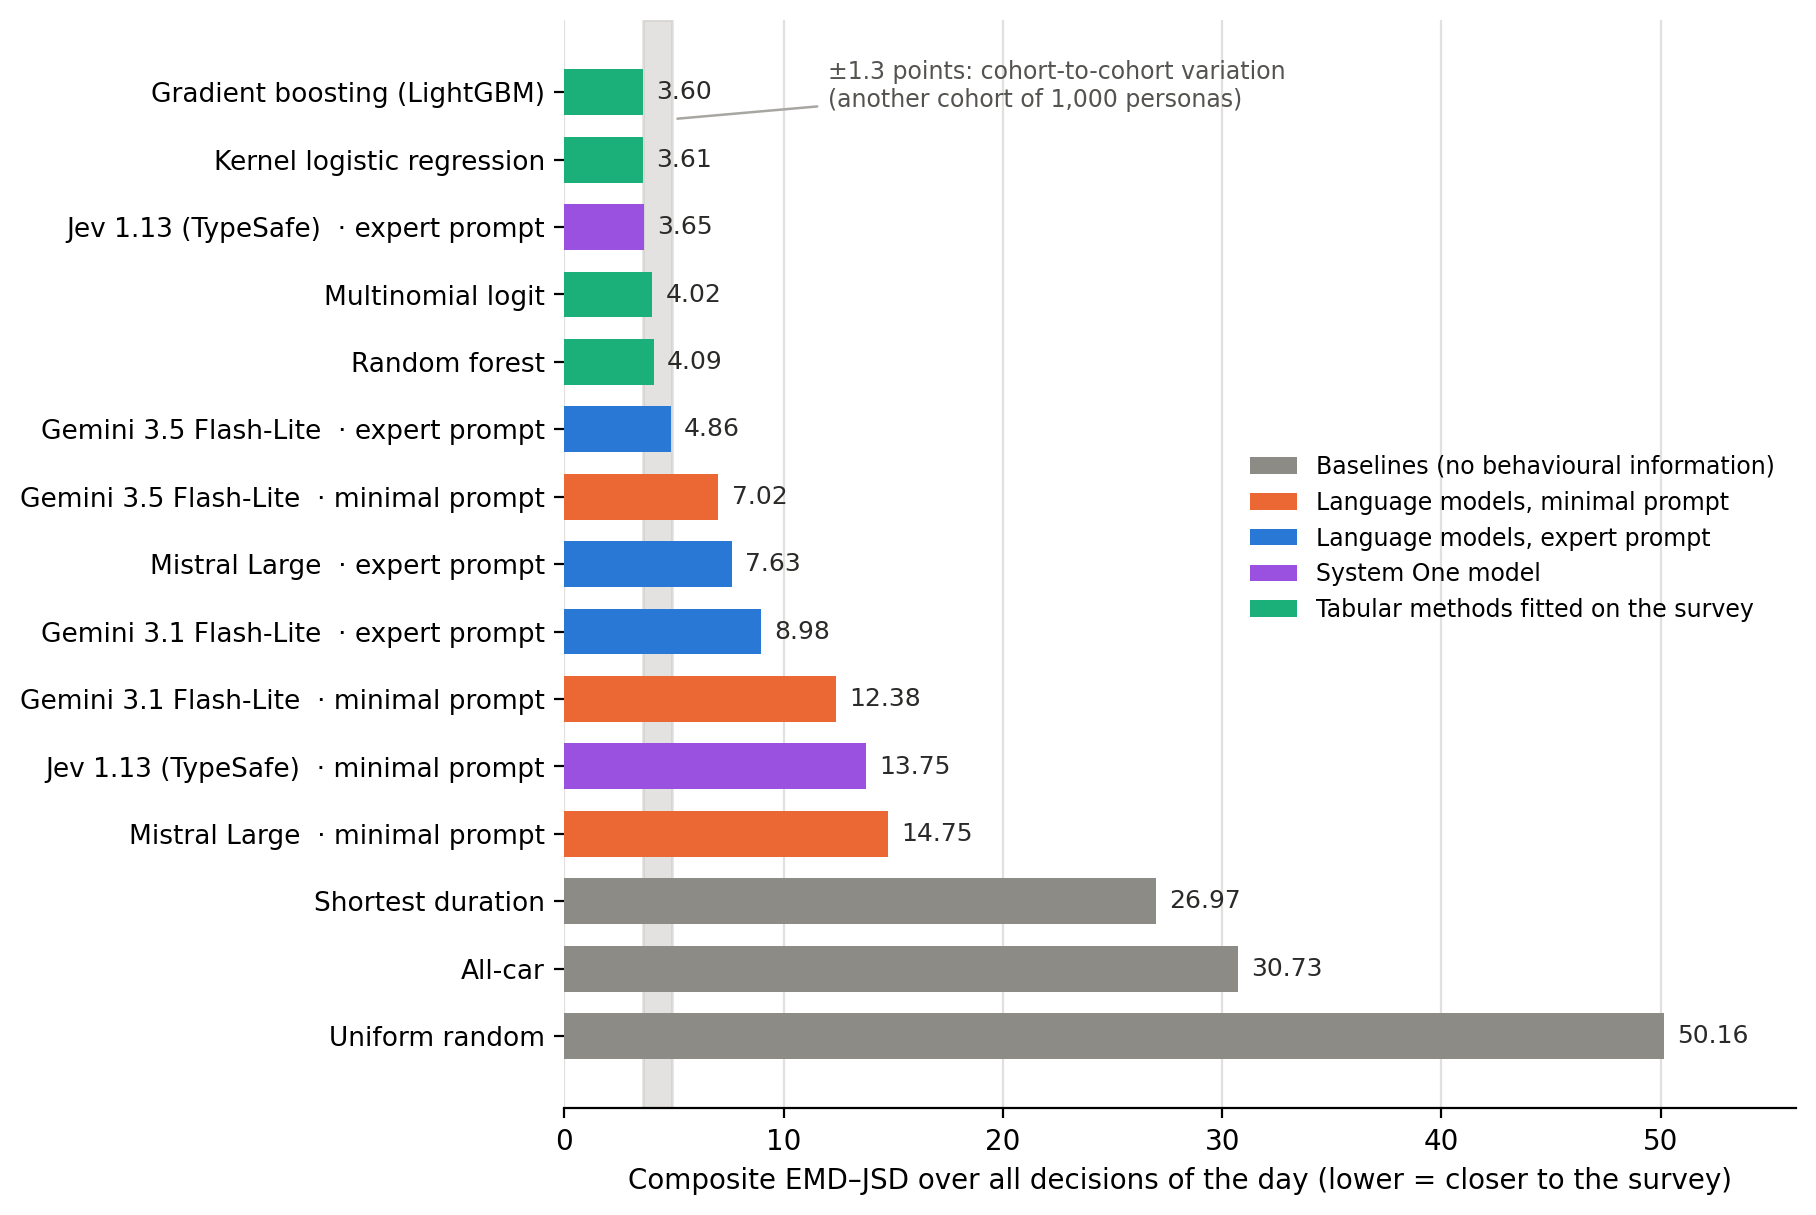
\includegraphics[width=\textwidth]{images/ch6_echelle.png}
  \caption{Cinq groupes se séparent sur l'axe composite, et l'invite minimale présente déjà moins d'erreur que le plancher physique.}
  \Description{Graphique à barres horizontales. L'axe des x représente l'erreur composite EMD-JSD sur chaque décision de la journée, de zéro à gauche à un peu plus de cinquante à droite ; plus la valeur est faible, plus elle est proche de l'enquête. Quinze décideurs sont empilés en lignes et colorés par groupe, chaque barre portant sa valeur. Du meilleur au moins bon : gradient boosting 3,60, régression logistique à noyau 3,61, classificateur typé sous son invite experte 3,65, logit multinomial 4,02 et forêt aléatoire 4,09 ; puis Gemini 3.5 Flash-Lite sous invite experte à 4,86, Gemini 3.5 Flash-Lite sous invite minimale à 7,02, Mistral Large sous invite experte à 7,63, Gemini 3.1 Flash-Lite sous invite experte à 8,98, Gemini 3.1 Flash-Lite sous invite minimale à 12,38, classificateur typé sous invite minimale à 13,75 et Mistral Large sous invite minimale à 14,75 ; à l'extrême droite les trois planchers, plus courte durée à 26,97, tout-voiture à 30,73 et tirage aléatoire uniforme à 50,16. Une bande grise verticale d'environ 1,3 point marque la variation inter-cohortes.}
  \label{fig:scale}
\end{figure*}

L'invite minimale présente déjà moins d'erreurs que le meilleur des trois planchers. La moins bonne des quatre conditions sous invite minimale se situe à 14,8, contre 27,0 pour l'heuristique de durée minimale, qui sélectionne l'option la plus rapide proposée. Un modèle qui reçoit les faits d'un trajet, et aucun critère général, porte donc des informations comportementales. Ces informations ne sont pas celles que l'heuristique physique encode.

Sur deux versions d'une famille de modèles, le modèle de base pèse autant que l'instruction qu'il véhicule. Appliqué sans modification à un second modèle du même fournisseur, le texte expert laisse un écart composite de 4,15 points entre les deux, avec un intervalle de $+$2,99 à $+$5,43.

La réexécution d'une condition avec trois initialisations différentes modifie son score composite de façon moins marquée que la cohorte elle-même. La condition \texttt{gemini-3.5} optimisée obtient des scores de 4,86, 4,65 et 4,30 sur la même cohorte et le même ensemble d'évaluation. L'écart est de 0,56 point, pour une résolution de cohorte de $\pm$1,3 point. Deux autres conditions réexécutées de la même manière présentent des écarts de 0,05 et 0,24 point. Le signe de leur différence est le même pour les trois initialisations.

\subsection{Ce que le réglage influence et ce qu'il n'influence pas}
\label{sec:tuning}

Le réglage des critères généraux améliore chaque modèle de langage, davantage qu'une cohorte ne progresserait seule (Tableau~\ref{tab:gains}). Le gain apparié sur l'axe composite est de 2,27 points pour \texttt{gemini-3.5}, intervalle de $+$1,40 à $+$3,22, puis de 3,37 points pour \texttt{gemini-3.1} et de 7,25 pour \texttt{mistral-large}. Les neuf intervalles excluent zéro. Les gains varient de une fois et demie à cinq fois et demie la résolution de la cohorte.

\begin{table*}[tp]
  \caption{Gains appariés de l'invite experte par rapport à l'invite minimale, trois lectures, avec leur intervalle de confiance à 95\,\% entre crochets. Un gain positif correspond à une erreur plus faible.}
  \label{tab:gains}
  \begin{tabular}{lccc}
    \toprule
    Modèle de langage & Composite & Hors trajets à option unique & L1 sur les parts globales \\
    \midrule
    \texttt{gemini-3.5}    & 2,27 [1,40 ; 3,22] & 3,59 [2,45 ; 4,83]  & 10,2 [8,0 ; 12,5]  \\
    \texttt{gemini-3.1}    & 3,37 [2,45 ; 4,25] & 4,15 [3,09 ; 5,22]  &  8,6 [6,8 ; 10,6]  \\
    \texttt{mistral-large} & 7,25 [5,90 ; 8,67] & 8,63 [7,15 ; 10,28] & 18,0 [13,5 ; 22,4] \\
    \bottomrule
  \end{tabular}
\end{table*}

Ces gains proviennent d'un texte optimisé, et son cheminement n'est pas unique. Chaque mutation déplace plusieurs strates simultanément, dans les deux sens. La procédure ne conserve que les individus dont le mode surreprésenté diminue.

Ce texte crée une pente plutôt qu'un changement de niveau (Figure~\ref{fig:distance}). Sur une distance inférieure à un kilomètre, la part de voiture de \texttt{gemini-3.5} reste stable : 9,7\,\% avant ajustement et 10,1\,\% après. Entre un et cinquante kilomètres, elle augmente de six à sept points dans chaque tranche. L'agent ajusté présente alors une erreur moindre sur la distance que toute référence tabulaire : 14,2 points pondérés contre 16,8 pour la forêt aléatoire. La distance est la seule dimension que l'agent gère.

\begin{figure}[tbp]
  \centering
  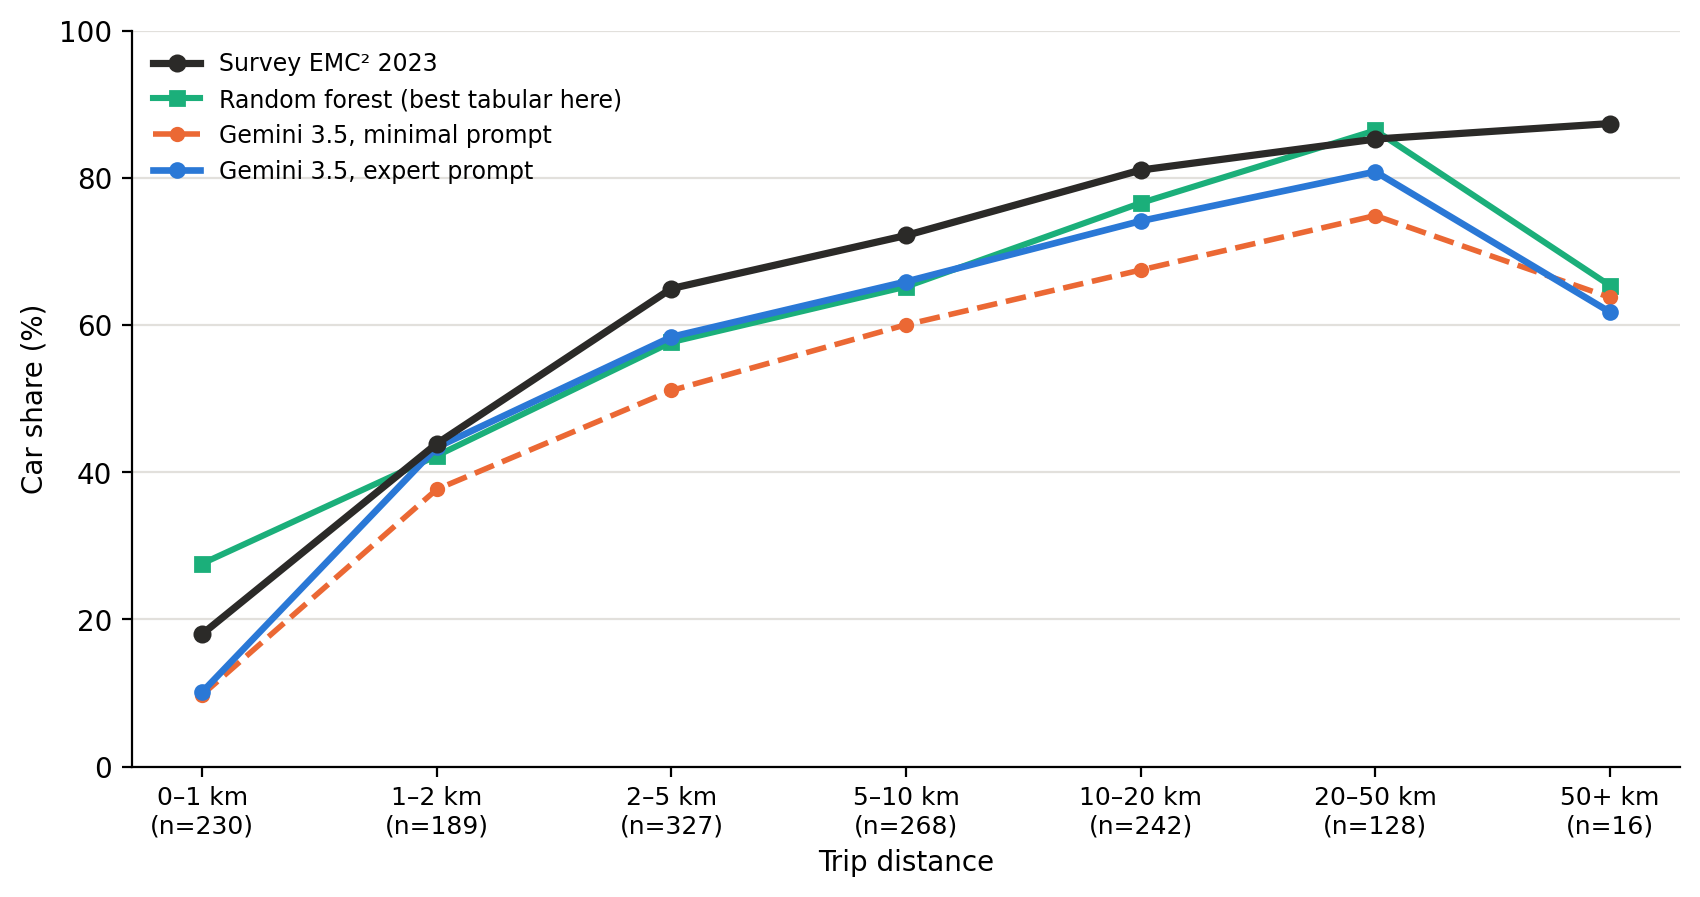
\includegraphics[width=\columnwidth]{images/ch6_distance.png}
  \caption{Le réglage confère à l'agent une pente en fonction de la distance, tandis que les trajets les plus courts restent là où l'invite minimale les a laissés.}
  \Description{Graphique linéaire à quatre séries. L'axe horizontal porte sept tranches de distance de trajet, de zéro à un kilomètre jusqu'à plus de cinquante kilomètres, chacune étiquetée avec son nombre de trajets. L'axe vertical est la part modale de la voiture en pourcentage, de zéro à cent. La courbe de l'enquête monte de 18 pour cent sur la tranche la plus courte à environ 87 pour cent sur la plus longue. L'agent sous invite minimale est le plus bas partout, d'environ 10 pour cent à 75 pour cent. L'agent sous invite experte part des mêmes 10 pour cent mais monte plus vite, rejoignant la forêt aléatoire à partir de deux kilomètres et restant cinq à dix points sous l'enquête.}
  \label{fig:distance}
\end{figure}

Deux erreurs coexistent chez le même décideur, et l'ajustement n'en corrige qu'une. Les trois modèles de langage situent la part de vélo entre 6,8 et 8,1\,\%, alors que l'enquête enregistre 4,1\,\%. Ce texte la modifie de moins d'un point et fait baisser la part des transports en commun de quatre à onze points. Une strate résiste à tous les décideurs : les 15--19 ans (Annexe F).

\subsection{La délibération ne décide pas}
\label{sec:deliberation}

Le classificateur dactylographié atteint la bande des quatre références tabulaires. Son score composite sur la seconde cohorte est \textbf{[c2, score composite hors échantillon du classificateur dactylographié]}, contre 3,60 à 4,09 points pour les quatre références tabulaires. Les différences appariées par rapport à ces quatre références sont \textbf{[c2, quatre différences appariées avec leurs intervalles à 95\,\%]}.

Un décideur qui ne rédige aucun texte obtient un score dans la même bande que ceux qui rédigent une justification. Ce qui aide, c'est donc la lecture du trajet, et non les phrases produites après le choix. La délibération verbalisée n'a rien apporté à la fidélité globale ici. Nous l'affirmons comme un résultat sur ce banc d'essai, et non comme une propriété des modèles de langage.

Pour une charge égale de 23\,026 décisions, le classificateur coûte 1,06 dollar contre 49,28, soit un facteur d'environ cinquante.

\subsection{L'agrégat ne renseigne pas l'individu}
\label{sec:individual}

L'agent optimisé et le modèle à gradient boosté se situent dans la résolution de cohorte l'un de l'autre et divergent encore sur un trajet sur trois. Ils attribuent leur probabilité la plus élevée à un mode différent pour 30,3\,\% des trajets, comptabilisés lorsque les deux ont vu au moins deux options. Cela compare les distributions, et non le mode tiré par chacun. Entre deux méthodes tabulaires, le même chiffre varie de 8,4 à 11,0\,\%. Deux agents diffèrent également quatre fois plus que deux modèles tabulaires sur l'ensemble de la distribution, avec une distance médiane de 40,0 points contre 9,8.

Les jours déclarés de l'enquête, l'agent désigne le mode déclaré légèrement moins souvent que les références tabulaires (Tableau~\ref{tab:unit}). L'audit porte sur 9\,621 trajets de 2\,930 répondants, chacun effectuant le trajet selon le mode déclaré. L'agent optimisé atteint une précision de 67,6\,\% contre 71,5\,\% pour le modèle à gradient boosté, soit un écart de 3,87 points (intervalle : $-$5,47 à $-$2,28). Son écart avec le modèle logit multinomial est significatif, tant en termes de précision que d'entropie croisée.

\begin{table}[tbp]
  \caption{Accord au niveau unitaire sur les jours déclarés, six décideurs. Précision et rappel (\%), entropie croisée sur les 5\,229 décisions prises par chaque décideur (à valeurs distribuées).}
  \label{tab:unit}
  \small
  \setlength{\tabcolsep}{4pt}
  \begin{tabularx}{\columnwidth}{@{}Lrrrr@{}}
    \toprule
    Décideur & \multicolumn{1}{c}{Préc.} & \multicolumn{1}{c}{Entr.} & \multicolumn{1}{c}{Rap.} & \multicolumn{1}{c}{Rap.} \\
             &                           & \multicolumn{1}{c}{crois.} & \multicolumn{1}{c}{vélo} & \multicolumn{1}{c}{marche} \\
    \midrule
    Gradient boosté                      & 71,5 & 0,299 & 20,4 & 63,4 \\
    Logit multinomial                    & 68,6 & 0,358 & 18,3 & 60,0 \\
    Durée minimale                       & 68,1 & ---   & 25,8 & 19,2 \\
    Invite experte, \texttt{gemini-3.5}  & 67,6 & 0,341 & 22,5 & 47,2 \\
    Invite minimale, \texttt{gemini-3.5} & 64,8 & 0,384 & 24,1 & 44,2 \\
    Invite experte, classificateur typé  & 64,7 & 0,464 & 18,1 & 56,3 \\
    \bottomrule
  \end{tabularx}
\end{table}

Le classificateur typé présente une précision individuelle inférieure au seuil minimal pour l'ensemble des véhicules. Il atteint 64,7\,\% là où le plancher atteint 66,7\,\%, soit un écart de 2,04 points (intervalle : $-$3,78 à $-$0,29). Les deux phrases suivantes se basent sur l'invite experte de \texttt{gemini-3.5}, et non sur celle du classificateur lui-même \textbf{[À déterminer]}. Aucune comparaison appariée ne le distingue des quatre références tabulaires sur le composite. Les deux autres lectures agrégées le placent derrière la régression à noyau et la forêt aléatoire. Sa probabilité est plus élevée pour la marche que pour les transports en commun. Le rappel pour la marche est de 56,3\,\%, contre \textbf{[À déterminer, environ 44\,\% sur la Figure~\ref{fig:audit-modes}, valeur exacte dans l'annexe I]} pour les transports en commun. La répartition agrégée masque cette inversion. Une population peut donc reproduire la répartition modale d'un territoire tout en commettant plus d'erreurs sur les trajets individuels qu'une règle qui ne tient pas compte de ces erreurs.

\begin{figure}[tbp]
  \centering
  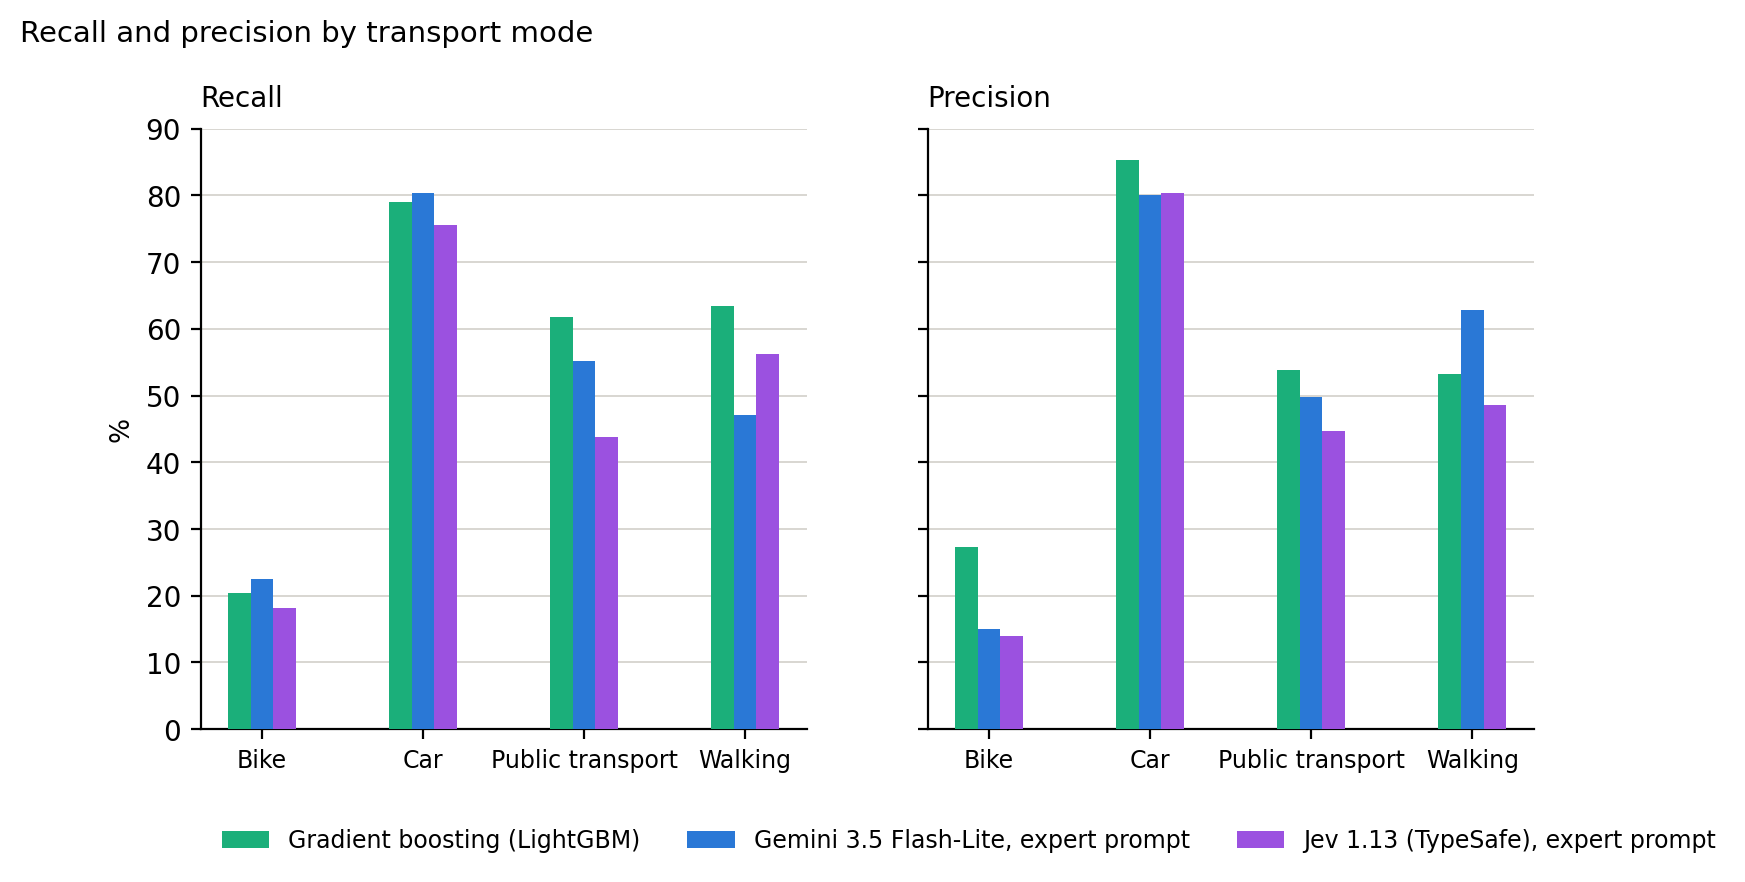
\includegraphics[width=\columnwidth]{images/ch6_audit_modes.png}
  \caption{Rappel et précision par mode : le classificateur typé remplace les transports en commun par la marche et la répartition agrégée ne reflète pas ce changement.}
  \Description{Deux panneaux de barres groupées, rappel à gauche et précision à droite. Dans chaque panneau, l'axe horizontal porte les quatre modes (vélo, voiture, transports en commun et marche), et l'axe vertical un pourcentage de zéro à quatre-vingt-dix. Trois barres par mode : gradient boosting, invite experte sur Gemini 3.5 Flash-Lite, et classificateur typé sous invite experte. Sur le rappel, le classificateur typé est le plus bas sur le vélo et les TC (environ 18 et 44 pour cent), et au-dessus de l'agent génératif sur la marche (56 pour cent contre 47). Sur la précision, la relation s'inverse sur la marche.}
  \label{fig:audit-modes}
\end{figure}

Ces quatre observations sont valables pour la journée ordinaire décrite par l’enquête. Une enquête ne recense aucune autre journée, et la section suivante aborde ce cas de figure pour un événement qu’aucune variable ne permet de modéliser.

% =====================================================================
% chapters/06_Non_tabulated.tex — rendu LaTeX de ../traductions/06_non_tabulated.en_brut.txt (23 septembre 2026)
% Section 6 de la VERSION FRANÇAISE de l'article court. \input depuis main.tex, après 05_Results.tex.
% Ce fichier DÉFINIT \label{sec:nontabulated} et \label{sec:mechanism}.
% Figure : une, \columnwidth (ch7_propension_quotidienne.png), légende AU-DESSOUS.
% Tableau : un, tab:offered, \columnwidth, légende AU-DESSUS, booktabs.
% Rendu mot pour mot de la traduction fournie par l'auteur.
% =====================================================================

\section{Le régime non tabulé : un événement impliquant un seul agent et retracé jusqu'à la décision}
\label{sec:nontabulated}

Cette section décrit un événement pour lequel aucune variable n’est enregistrée, chez un agent donné, depuis son entrée en mémoire jusqu’aux décisions qu’il a influencées.

\subsection{Ce que les 21 variables ne contiennent pas}
\label{sec:variables-gap}

Aucune des 21 variables n’enregistre ce qu’une personne a vécu la veille, ni ce qu’elle a lu ce matin. Un décideur qui ne reçoit que ces informations ne peut répondre à aucune autre question. Sa prédiction le lendemain matin d’un incident est identique à celle de la veille, par identité plutôt que par mesure.

\subsection{Le mécanisme}
\label{sec:mechanism}

Un événement entre dans la mémoire de l’agent à deux moments différents. Un événement vécu y entre après le voyage qui l’a produit, et un événement lu y entre au réveil. À l’entrée, l’agent évalue l’événement sur une échelle de gravité à cinq niveaux et lui attribue une valence : subi ou bienvenu. L’évaluation est propre à l’agent et comparée à son profil ; ainsi, un même incident n’a pas le même impact sur deux agents. La gravité détermine à elle seule la durée de fonctionnement de la mémoire.

Un événement évalué se propage au-delà de son propriétaire, à travers le foyer, le soir.

Un effet prend fin de deux manières, que la mesure permet de distinguer. Il prend fin par contradiction lorsque l'agent effectue à nouveau le trajet et qu'aucun événement ne se reproduit, et par usure lorsque la mémoire cesse d'être utilisée.

Deux maillons de cette chaîne sont la génération de texte. L'un consiste à consigner la trace de ce qui vient de se produire, et l'autre à maintenir la croyance qui en découle. Le modèle de langage évalue également la gravité, et ce maillon ne relève pas de la génération de texte. L'évaluation constitue un niveau dans une grille fermée, qu'un classificateur typé peut renvoyer. La question de savoir s'il pourrait également produire les deux maillons écrits reste ouverte et une étude approfondie permettrait de trancher.

\subsection{Configuration}
\label{sec:setup}

Nous jouons un agent deux fois, en tant qu'agent exposé et agent témoin, et nous mesurons l'écart entre les deux exécutions. L'incident est une panne de moteur qui impose un retard d'une demi-heure à un trajet en voiture. Les deux exécutions maintiennent la mémoire activée. La voiture reste proposée le lendemain matin ; ce que nous mesurons ici est donc un arbitrage. \textbf{[À confirmer --- Campagne en cours]}

Les avis sont recueillis en dehors de toute prise de décision, selon six critères définis, à quatre étapes clés. Le critère relatif à l'environnement, qui n'est concerné par aucun incident, sert de question de contrôle.

\subsection{Résultats}
\label{sec:traced-results}

Bien que la voiture soit proposée aussi souvent qu'avant la panne, elle n'est plus prise. L'agent exposé la prend neuf fois sur dix avant la panne, et trois fois sur dix après. L'agent de contrôle maintient son taux tout au long de la période.

\begin{table}[tbp]
  \caption{Voiture prise lorsqu'elle est proposée, agent exposé et agent de contrôle.}
  \label{tab:offered}
  \begin{tabular}{@{}lrr@{}}
    \toprule
    Période & Agent exposé & Agent de contrôle \\
    \midrule
    Avant la panne  & 94\,\% (34/36) & 90\,\% (28/31) \\
    Après la panne  & 32\,\% (12/38) & 92\,\% (45/49) \\
    Après le retour & 88\,\% (35/40) & 87\,\% (40/46) \\
    \bottomrule
  \end{tabular}
\end{table}

La propension quotidienne à utiliser la voiture chute le jour de l'incident et remonte quinze jours plus tard (Figure~\ref{fig:propensity}). Elle passe de 90\,\% la veille à 40\,\% ce jour-là, puis oscille entre 5\,\% et 52\,\%. Elle rejoint la plage de l'agent de contrôle, qui se situe toujours entre 65\,\% et 90\,\%, le 15 avril.

\begin{figure}[tbp]
  \centering
  
\includegraphics[width=\columnwidth]{images/ch7_propension_quotidienne.png}
  \caption{L'effet dure exactement aussi longtemps que le souvenir reste dans l'invite.}
  \Description{Deux séries temporelles quotidiennes de la probabilité attribuée par l'agent à la voiture, en pourcentage, sur environ six semaines de mi-mars à fin avril. L'agent exposé et le témoin évoluent ensemble au-dessus de 65 pour cent jusqu'au jour de la panne, marqué par une ligne verticale en tiretés. La série exposée s'effondre alors entre 5 et 52 pour cent pendant quinze jours, tandis que le témoin continue d'osciller entre 65 et 90 pour cent. Une ligne verticale en pointillés marque le jour où le récit de la panne quitte le contexte de décision, et la série exposée rejoint la bande témoin deux jours plus tard, le 15 avril, et y reste.}
  \label{fig:propensity}
\end{figure}

Les quatre voies par lesquelles le passé influence une décision peuvent être distinguées, et la trace indique celle qui a produit cet effet. Le compte rendu de l'incident apparaît dans le bloc des changements récents, dans 75 des 376 invites de décision. Il y reste du jour de l'incident jusqu'au quinzième jour suivant. Cette durée découle de la gravité. \textbf{[À confirmer --- La campagne en cours indique le contenu des trois autres itinéraires.]}

La mesure distingue les deux manières dont un effet peut prendre fin, et celui-ci a pris fin par usure. L'agent a pris la voiture douze fois pendant la période. \textbf{[À confirmer --- à ce stade, aucune contradiction avec la croyance née de l'échec. Ajouter une expérience ?]} Le compte quitte les invites de décision après le 13 avril, et la propension rejoint la bande de contrôle le 15 avril. Deux sources indépendantes fournissent ces dates, le texte envoyé au modèle et les probabilités qu'il a renvoyées.

Les opinions déclarées diminuent après l'échec et reviennent. Cinq des six critères relatifs à la voiture chutent à l'étape suivante, la sécurité passant de 8 à 3 sur une échelle de dix. Les cinq ont retrouvé leur valeur initiale aux deux étapes suivantes. Le critère environnemental reste à 3 tout au long de la période, et l'agent de contrôle ne modifie aucun des six critères. Les deux agents dérivent sur les quatre autres modes sans schéma commun, la voiture étant le seul mode qui les distingue.

\textbf{Une seconde expérience utilise le même canal pour transmettre des informations qui ne sont que lues. Actuellement en cours, elle oppose cinq articles de presse toulousains datés à vingt panneaux écrits avant tout appel au modèle (Annexe E).}

Le chemin tracé ici repose sur un agent et un événement. Nous nous intéressons au chemin plutôt qu'à son amplitude.

% =====================================================================
% chapters/07_Implications.tex — rendu LaTeX de ../traductions/07_implications.en_brut.txt (23 septembre 2026)
% Section 7 de la VERSION FRANÇAISE de l'article court, la dernière. \input depuis main.tex, après 06_Non_tabulated.tex.
% Ce fichier DÉFINIT \label{sec:implications}.
% Il RÉFÉRENCE sec:mechanism (Section 6.2), sec:individual (Section 5.4) et sec:nontabulated (Section 6).
% Citation : chopra2024limits.
% Rendu mot pour mot de la traduction fournie par l'auteur.
% =====================================================================

\section{Implications, limites, conclusion}
\label{sec:implications}

La journée ordinaire et l'événement analysé nous éclairent sur la conception d'un agent de mobilité et sur ce que nous ne pouvons pas affirmer.

\subsection{Ce que ces résultats révèlent sur l'architecture}
\label{sec:architecture-implication}

Avec les modèles utilisés, le coût d'une journée simulée détermine les limites de la réflexion. Une journée de semaine, pour plus de 1\,000 personas, sollicite le modèle de langage 2\,108 fois et consomme 3 millions de jetons, avec la mémoire désactivée. L'activation de la mémoire ajoute environ 2,5 millions de jetons. À l'échelle des 453 communes couvrant l'enquête, une journée simulée nécessiterait 2,9 millions de requêtes, pour un coût de 2,6 à 4,2 milliards de jetons. Une réponse publiée concernant ce coût interroge le modèle une fois par archétype comportemental plutôt qu'une fois par agent \citep{chopra2024limits}. Huit millions d'agents y fonctionnent avec une centaine d'archétypes, les agents ayant les mêmes attributs partageant une même réponse. Cette économie nous est inaccessible ici, car un événement non tabulé correspond précisément à ce qu'aucun attribut n'enregistre.

Nos mesures suggèrent une division du travail par régime plutôt qu'un décideur unique partout. Nous proposons cette solution comme implémentation possible, bien qu'elle ne soit pas encore mise en œuvre dans notre système. Une étape déterministe supprimerait les options qu'une personne ne peut pas choisir, faute de permis, d'un véhicule stationné ailleurs ou d'un itinéraire. Un modèle tabulaire contiendrait alors le régime nominal. Un classificateur typé évaluerait la gravité de l'événement, une tâche actuellement assurée par le modèle de langage. Il indiquerait également si le cas a quitté ce régime (Section~\ref{sec:mechanism}) et choisirait l'itinéraire le cas échéant. Le modèle de langage recevrait ce qu'aucune variable ne contient et l'écrirait en mémoire.

La deuxième étape impose un choix que nos mesures ne permettent pas de trancher. Un modèle tabulaire contient les deux échelles, bien qu'il n'existe pas avant l'enquête qui lui correspond. Le classificateur typé n'a pas besoin d'une telle enquête pour fonctionner et correspond toujours à la bande tabulaire au niveau agrégé. Une enquête est essentielle pour le calibrer, et sans elle, son réalisme repose sur des pondérations établies ailleurs plutôt que sur une analyse du territoire. Ces pondérations proviennent d'un corpus global, et rien n'y est adapté aux habitudes, aux spécificités ou à la culture d'un lieu. De plus, pour les trajets individuels, le modèle se situe en dessous du seuil minimal de fonctionnement en voiture (Section~\ref{sec:individual}). Une architecture le plaçant au niveau nominal permettrait d'obtenir une fidélité globale à moindre coût, mais au détriment de la fidélité individuelle. Un décideur qui prend en compte le contexte, n'a besoin d'aucune enquête locale, conserve la valeur globale et dépasse ce seuil minimal n'existe pas dans nos mesures. Cet article laisse le problème ouvert. Nous n'estimons pas la part des trajets que chaque étape effectuerait.

\subsection{Limites}
\label{sec:limitations}

Quatre limites encadrent la portée de ces mesures. Les références tabulaires sont basées sur 39\,203 trajets d'enquête pour lesquels les agents n'ont effectué aucune lecture ; aucun résultat ne compare donc ici deux décideurs disposant d'informations égales. La portée de ce modèle est plus restreinte. Un décideur qui se base uniquement sur les 21 variables ne peut réagir à un événement qu'aucune d'entre elles ne relate, quelle que soit sa précision. Nous montrons qu'un agent réagit à un tel événement. Nous ne montrons pas qu'il prend une meilleure décision. L'incident de la section~\ref{sec:nontabulated} permet de garder la voiture utilisable, alors qu'une véritable panne de moteur l'immobiliserait. Notre convention de recherche interdit la transmission des microdonnées de l'enquête ; par conséquent, la réestimation de nos références tabulaires nécessite l'obtention de l'enquête dans les mêmes conditions. La référence elle-même constitue la quatrième limite. L'enquête décrit un jour de semaine hors vacances scolaires, recueilli à partir des souvenirs des répondants concernant la veille, pour les résidents âgés de cinq ans et plus. Rien ici ne s'applique donc aux week-ends, aux périodes de vacances ou aux déplacements non déclarés par les répondants.

\subsection{Conclusion}
\label{sec:conclusion}

Nous nous sommes interrogés sur l'apport de la délibération verbalisée à la simulation urbaine et sur sa place au sein d'un agent de mobilité. Peut-il interpréter des signaux absents des colonnes de l'enquête, concernant le contexte ou le vécu d'une personne ? Elle ne mérite pas cette place au quotidien.

Ce quotidien est celui que décrit l'enquête certifiée de 2023 sur les déplacements des ménages à Toulouse, telle que rapportée par ses répondants. Un agent génératif calibré atteint les modèles tabulaires ajustés à partir de cette enquête sans les parcourir. Un classificateur dactylographié qui n'écrit aucun texte atteint le même résultat, pour un cinquantième du coût. Aucun de ces résultats ne justifie des milliards de jetons, ni la latence qu'ils imposent, même avec des prix en baisse qui réduisent les deux côtés de ce ratio. La délibération justifie son coût sur ce que l'enquête ne tabule pas, et c'est une architecture hybride qui la confine à cela. Un événement qu'aucune variable ne porte entre dans la mémoire de l'agent et influence ses choix au fil du temps, puis disparaît. Nous montrons par quel canal, dans un cas suivi de bout en bout, au sein d'une population calibrée à partir de cette enquête.

Deux questions restent en suspens. Nous poursuivons la recherche du décideur manquant, celui qui pourrait détenir les deux échelles sans enquête locale. La campagne de presse, qui utilise le même canal que l'agent pour diffuser des informations qu'il ne fait que lire, n'a pas repris.


%%%%%%%%%%%%%%%%%%%%%%%%%%%%%%% ANNEXES %%%%%%%%%%%%%%%%%%%%%%%%%%%%%%%%%%%%%%%%%

%%%%%%%%%%%%%%%%%%%%%%%%%%%%%%%%%%%%%%%%%%%%%%%%%%%%%%%%%%%%%%%%%%%%%%%%

%%% Remerciements : a remplir avant la version non anonyme. Le gabarit livrait ici un
%%% texte d'exemple ; il est retire (consigne R14, aucun placeholder dans le texte livre).
%%% \begin{acks} ... \end{acks}

%%%%%%%%%%%%%%%%%%%%%%%%%%%%%%%%%%%%%%%%%%%%%%%%%%%%%%%%%%%%%%%%%%%%%%%%

%%% The next two lines define, first, the bibliography style to be 
%%% applied, and, second, the bibliography file to be used.

\bibliographystyle{ACM-Reference-Format} 
\bibliography{sample}

%%%%%%%%%%%%%%%%%%%%%%%%%%%%%%%%%%%%%%%%%%%%%%%%%%%%%%%%%%%%%%%%%%%%%%%%

\end{document}

%%%%%%%%%%%%%%%%%%%%%%%%%%%%%%%%%%%%%%%%%%%%%%%%%%%%%%%%%%%%%%%%%%%%%%%%

